\documentclass[aspectratio=169]{beamer}
\usetheme{Madrid}
\usecolortheme{seahorse}
\usepackage[spanish]{babel}
\usepackage[utf8]{inputenc}
\usepackage[T1]{fontenc}
\usepackage{amsmath, amssymb}
\usepackage{booktabs}
\usepackage{graphicx}

\title{Planificación y Operación de Sistemas Eléctricos de Potencia}
\subtitle{Modelos de optimización, casos de estudio y análisis de resultados}
\author{Asignatura: Planificación y Operación de SEP}
\institute{ESPOCH · Electricidad}
\date{}

\begin{document}

\begin{frame}
  \titlepage
\end{frame}

\begin{frame}{Propósito de la asignatura}
  \begin{itemize}
    \item Comprender modelos de optimización aplicados a sistemas eléctricos de potencia.
    \item Formular problemas de operación y planificación mediante conjuntos, parámetros, variables, objetivo y restricciones.
    \item Analizar casos de estudio y resultados computacionales.
    \item Relacionar decisiones de corto plazo con decisiones de inversión de largo plazo.
  \end{itemize}
\end{frame}

\begin{frame}{Horizontes temporales}
  \begin{center}
    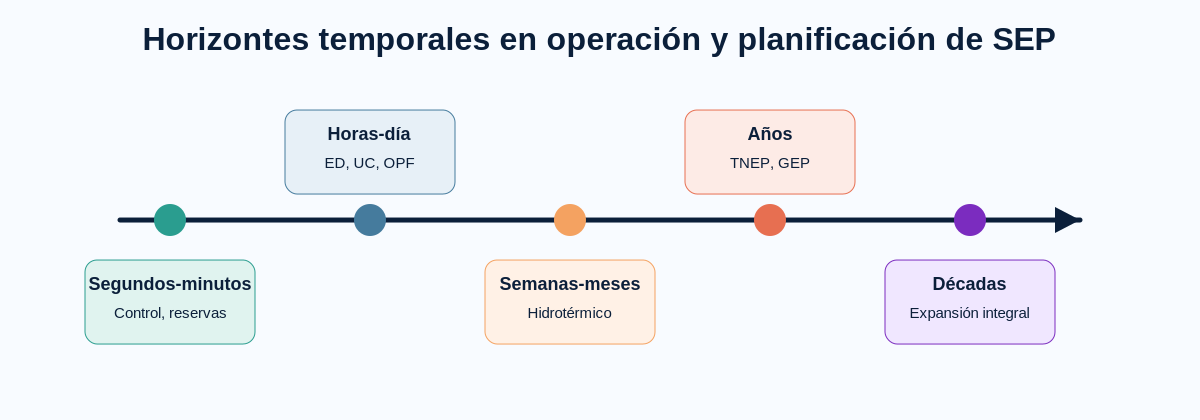
\includegraphics[width=0.95\linewidth]{../../docs/assets/img/horizontes_temporales_sep.png}
  \end{center}
\end{frame}

\begin{frame}{Clasificación general}
  \begin{center}
    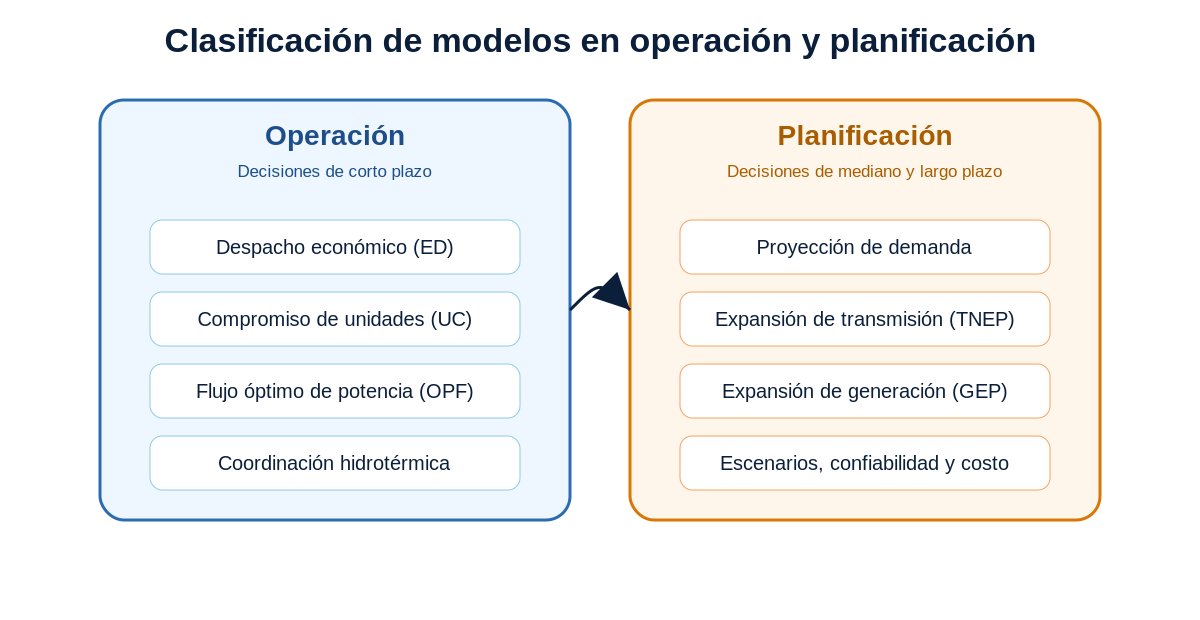
\includegraphics[width=0.90\linewidth]{../../docs/assets/img/clasificacion_operacion_planificacion.png}
  \end{center}
\end{frame}

\begin{frame}{Bloques del repositorio}
  \begin{center}
    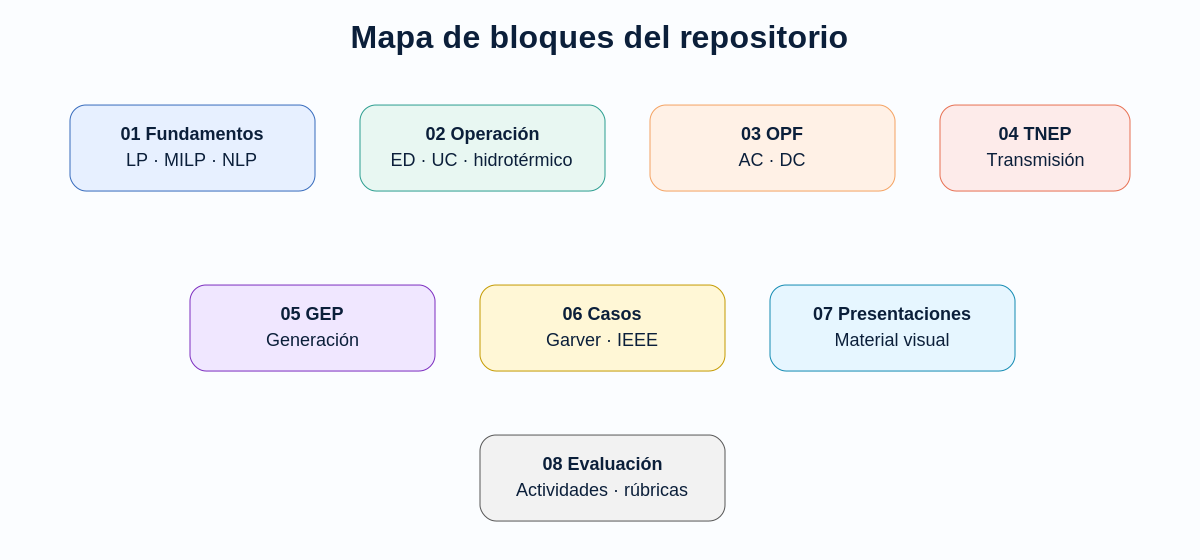
\includegraphics[width=0.88\linewidth]{../../docs/assets/img/mapa_bloques_repositorio.png}
  \end{center}
\end{frame}

\begin{frame}{Estructura de una formulación matemática}
  Todo modelo de optimización de la asignatura se describe mediante:
  \begin{enumerate}
    \item Conjuntos e índices.
    \item Parámetros técnicos y económicos.
    \item Variables de decisión.
    \item Función objetivo.
    \item Restricciones operativas, físicas o de inversión.
  \end{enumerate}
\end{frame}

\begin{frame}{Ejemplo: despacho económico}
  \textbf{Objetivo:} minimizar el costo de generación para atender una demanda.
  \[
    \min \sum_{g\in \mathcal{G}} c_g P_g
  \]
  sujeto a:
  \[
    \sum_{g\in\mathcal{G}} P_g = D
  \]
  \[
    P_g^{\min} \leq P_g \leq P_g^{\max} \qquad \forall g\in\mathcal{G}
  \]
\end{frame}

\begin{frame}{Ejemplo: expansión de generación}
  \textbf{Decisión principal:} determinar nueva capacidad de generación por tecnología y periodo.
  \[
    \min \sum_{t\in\mathcal{T}} \sum_{k\in\mathcal{K}} IC_{k,t} x_{k,t}
    + \sum_{t\in\mathcal{T}} \sum_{b\in\mathcal{B}} \sum_{g\in\mathcal{G}} C_g p_{g,b,t}
  \]
  El modelo combina inversión, operación representativa, reserva y atención de demanda.
\end{frame}

\begin{frame}{Casos de estudio}
  \begin{itemize}
    \item Garver 6 barras: TNEP y GEP didáctico.
    \item IEEE 14 barras: análisis de red y OPF.
    \item IEEE 24 RTS: operación horaria, confiabilidad y planificación.
    \item Sistemas reducidos: formulación básica y validación manual.
  \end{itemize}
\end{frame}

\begin{frame}{Actividad de clase}
  \textbf{Caso:} Garver 6 barras.\\[0.5em]
  El estudiante debe:
  \begin{itemize}
    \item Identificar demanda, tecnologías candidatas y límites.
    \item Formular restricciones principales.
    \item Ejecutar el caso indicado por el docente.
    \item Comparar escenario base y escenarios modificados.
    \item Elaborar conclusiones técnicas.
  \end{itemize}
\end{frame}

\begin{frame}{Evaluación}
  \begin{table}
    \centering
    \begin{tabular}{ll}
      \toprule
      Evidencia & Criterio principal \\
      \midrule
      Formulación & Coherencia matemática \\
      Ejecución & Reproducibilidad del caso \\
      Interpretación & Relación técnica-económica \\
      Sensibilidad & Comparación de escenarios \\
      Comunicación & Claridad y trazabilidad \\
      \bottomrule
    \end{tabular}
  \end{table}
\end{frame}

\begin{frame}{Cierre}
  La operación y la planificación se estudian como un conjunto articulado de problemas. Un resultado de inversión debe ser analizado junto con criterios de operación, red, confiabilidad, costo y escenarios futuros.
\end{frame}

\end{document}
